% For submission and review of your manuscript please change the command to 
\documentclass[manuscript, screen]{acmart}
% When submitting camera ready or to TAPS, please change the command to 
% \documentclass[sigconf]{acmart}

\pagestyle{plain}

\usepackage{xspace}
\usepackage{siunitx}
\DeclareSIUnit{\fps}{fps}
\usepackage[inline]{enumitem}
\usepackage{multicol}
\usepackage{multirow}
\usepackage{graphicx} % Ensure graphicx is included for figures

\newcommand{\etal}{\emph{et~al.\xspace}}
\newcommand{\ie}{\emph{i.e.}, }
\newcommand{\eg}{\emph{e.g.}, }
\newcommand{\etc}{\emph{etc.\xspace}}
\newcommand{\vxv}[2]{$#1\!\times\!#2$}

\AtBeginDocument{%
  \providecommand\BibTeX{{%
    Bib\TeX}}}

% Rights management information. 
% \copyrightyear{2025}
% \acmYear{2025}
% \setcopyright{acmcopyright}
% \acmConference[TOMM '25]{ACM Transactions on Multimedia Computing, Communications, and Applications}{TBD 2025}{TBD}
% \acmBooktitle{ACM Transactions on Multimedia Computing, Communications, and Applications (TOMM '25)}
% \acmDOI{TBD}
% \acmISBN{TBD}

\begin{document}

\title[PointStream]{PointStream: A Hybrid Semantic Codec with Generative Reconstruction for Live Video Streaming}

\author{Emanuele Artioli}
\email{emanuele.artioli@aau.at}
\orcid{0009-0007-9921-0006}
\affiliation{
  \institution{Alpen-Adria-Universitaet}
  \city{Klagenfurt}
  \state{Kaernten}
  \country{Austria}
}
\author{Daniele Lorenzi}
\email{daniele.lorenzi@aau.at}
\orcid{0000-0003-3689-6315}
\affiliation{
  \institution{Alpen-Adria-Universitaet}
  \city{Klagenfurt}
  \state{Kaernten}
  \country{Austria}
}
\author{Farzad Tashtarian}
\email{farzad.tashtarian@aau.at}
\orcid{0000-0002-5584-6690}
\affiliation{
  \institution{Alpen-Adria-Universitaet}
  \city{Klagenfurt}
  \state{Kaernten}
  \country{Austria}
}
\author{Christian Timmerer}
\email{christian.timmerer@aau.at}
\orcid{0000-0002-0031-5243}
\affiliation{
  \institution{Alpen-Adria-Universitaet}
  \city{Klagenfurt}
  \state{Kaernten}
  \country{Austria}
}

\begin{abstract}
As video resolutions and frame rates continue to rise, a key challenge in video streaming is maintaining high quality under constrained bandwidth. While recent work explores semantic compression, many approaches still transmit large amounts of pixel data or are unsuitable for live applications. We introduce PointStream, a hybrid, object-centric streaming framework designed for real-time video. PointStream classifies scenes based on background motion: scenes with complex motion are encoded with a traditional codec like AV1, while stable scenes (those with static or simple motion) are processed by our neural codec. For these stable scenes, the background is modeled as a single panoramic image, and its motion is described by a stream of homography matrices. The server then transmits only high-level information about dynamic foreground objects—such as poses and minimal appearance descriptors. Full frames are reconstructed on the client by warping the background panorama and using generative models to synthesize the foreground. This approach is demonstrated on a variety of content, with a focus on sports videos. Experiments show that PointStream achieves adequate perceptual quality (e.g., 60 VMAF) at bitrates under 200 Kbps, whereas state-of-the-art live codecs require 7 to 10 times more bandwidth to reach the same quality. The modular implementation and dataset will be made available upon acceptance.
\end{abstract}

\renewcommand{\shortauthors}{Emanuele Artioli, et al.}

\begin{CCSXML}
<ccs2012>
    <concept>
        <concept_id>10010147.10010178.10010224.10010245.10010252</concept_id>
        <concept_desc>Computing methodologies~Object identification</concept_desc>
        <concept_significance>500</concept_significance>
        </concept>
    <concept>
        <concept_id>10010147.10010178</concept_id>
        <concept_desc>Computing methodologies~Artificial intelligence</concept_desc>
        <concept_significance>500</concept_significance>
        </concept>
    <concept>
        <concept_id>10002951.10003227.10003251.10003255</concept_id>
        <concept_desc>Information systems~Multimedia streaming</concept_desc>
        <concept_significance>500</concept_significance>
        </concept>
    <concept>
        <concept_id>10010147.10010371.10010395</concept_id>
        <concept_desc>Computing methodologies~Image compression</concept_desc>
        <concept_significance>500</concept_significance>
        </concept>
</ccs2012>
\end{CCSXML}

\ccsdesc[500]{Computing methodologies~Object identification}
\ccsdesc[500]{Computing methodologies~Artificial intelligence}
\ccsdesc[500]{Information systems~Multimedia streaming}
\ccsdesc[500]{Computing methodologies~Image compression}

\keywords{HTTP adaptive streaming, Generative AI, Semantic Video Coding, Quality of Experience}

\maketitle

\section{Introduction}
Modern video codecs consume excessive bandwidth by encoding important motion with the same priority as irrelevant visual details--an increasingly critical inefficiency, given that video streaming is ubiquitous and accounts for 65\% of global Internet traffic~\cite{sandvine}. While traditional codecs like High Efficiency Video Codec (HEVC or H.265)~\cite{h265_overview} or AOMedia Video~1 (AV1)~\cite{av1_overview}, \etc ~employ compression techniques such as motion estimation to significantly reduce redundancy, they still encode full frames and treat them as sequences of blocks. As a result, they lack higher-level semantic understanding, give equal priority to imperceptible background changes, and fail to exploit predictable object appearance and movement. The ongoing shift to 4K (\vxv{3840}{2160}) resolution and beyond makes these inefficiencies more pronounced.

In contrast, the human visual system processes scenes with remarkable efficiency. Rather than uniformly parsing the entire visual field, the brain focuses attention on salient objects and motion, using peripheral vision to gather low-resolution contextual cues~\cite{cajar2016spatial}. Moreover, the brain leverages prior visual experience to anticipate familiar patterns, allowing it to infer and reconstruct missing or occluded information based on learned expectations~\cite{serences2006selective}. This combination of object-centric processing and predictive inference yields a far more efficient representation of dynamic environments than conventional video compression methods achieve.

Inspired by this efficiency, we propose {\em PointStream}, a novel hybrid codec for live video streaming that prioritizes semantically meaningful content. PointStream's pipeline begins by classifying scenes based on background motion. Scenes with complex, unpredictable motion are gracefully handed off to a traditional codec like AV1, ensuring that the system is never worse off than the standard alternative, save for a minor analysis overhead. For scenes with static or simple motion (e.g., pans or zooms), our neural codec takes over. It identifies and isolates objects of interest, encoding their motion into a lightweight representation of keypoints derived from pose estimation models. The background is modeled separately, either as a single static image or as a larger stitched panorama with corresponding transformation matrices. The client receives this compact data packet and uses generative models to reconstruct high-fidelity video frames. This approach differs from foveated streaming, which saves bandwidth by degrading the quality of the visual periphery. While effective, foveated methods can lead to a poor experience if the viewer's focus shifts unexpectedly to a low-quality region. PointStream avoids this by always preserving a high-quality background, ensuring a perceptually stable experience while still achieving significant bandwidth savings.

The primary contributions of this work include:
\begin{itemize}[topsep=0pt,itemsep=0pt,leftmargin=*]
\item \textbf{A hybrid semantic video codec} that intelligently routes video segments to either a traditional codec or our neural codec based on scene complexity, optimizing for both quality and efficiency.
\item \textbf{An efficient server-side pipeline} that uses modern deep learning models for object detection (YOLOv12), pose estimation (MMPose), and background modeling to create a low-bitrate semantic representation.
\item \textbf{A modular end-to-end system} designed for research, allowing for pluggable components and detailed performance instrumentation to facilitate ablation studies.
\end{itemize}

\section{Related Work}

\subsection{Traditional video coding and streaming}
Leveraging the Hypertext Transfer Protocol (HTTP) as a ubiquitous and interoperable foundation, HTTP Adaptive Streaming (HAS) delivers video content over the Internet under varying network conditions. HAS enables clients to switch between video qualities based on real-time measurements of network throughput and buffer levels. Adaptive Bitrate (ABR) control, typically implemented on the client side, represents the dominant strategy for streaming at scale~\cite{sani2017abr}. Standardized HAS variants, such as Dynamic Adaptive Streaming over HTTP (DASH)~\cite{Stockhammer2011} and HTTP Live Streaming (HLS)~\cite{AppleHLS}, partition videos into small HTTP-delivered segments and encode them at multiple quality levels. Clients select the version of each upcoming segment that best matches predicted network conditions, reducing rebuffering and enhancing the overall quality of experience~\cite{QoEWhitePaper}.

As video resolutions and streaming demands continue to rise, more advanced codecs emerge to improve compression efficiency. State-of-the-art standards such as Versatile Video Coding (VVC or H.266)~\cite{vvc_overview} and AV1~\cite{av1_overview} reduce bitrates by up to 50\% compared to their predecessors, HEVC and VP9~\cite{vp9_overview}, while maintaining similar visual quality. However, these gains come at the cost of significantly increased computational complexity, particularly during encoding, which limits their practicality for real-time or low-power applications. This trade-off prompts ongoing exploration of alternative compression techniques.

\subsection{Beyond traditional codecs}
Artificial intelligence (AI) techniques offer potential advancements in video streaming. AI-driven approaches enhance traditional codec pipelines by integrating AI modules that optimize specific components, such as rate control, motion estimation, or bitrate allocation, without altering the overall codec architecture~\cite{liu2020deep, lu2019dvc}. These hybrid methods improve compression efficiency and visual quality while remaining compatible with existing standards. In contrast, end-to-end neural video codecs replace the entire traditional pipeline with deep learning models that directly learn compact representations of video content from data~\cite{lu2019dvc, chen2021nerv}. While these fully learned systems match or even exceed the compression rates of conventional codecs, they introduce even higher computational complexity, particularly during encoding, which limits their practicality for real-time or resource-constrained scenarios.

As the computational complexity of modern video codecs continues to grow, especially on the encoding side, researchers explore ways to shift some of the processing load to the client. This shift leads to the development of techniques that enhance video quality after transmission, leveraging the increasing capabilities of consumer hardware. Notable examples include client-side frame interpolation~\cite{niklaus2020softmax, xu2019quadratic} and super-resolution~\cite{ledig2017photo}, which improve perceived visual quality independently of network conditions. These approaches represent a promising direction in research, optimize natively for the rapidly increasing capabilities of modern Graphics Processing Units (GPUs), and offer a practical way to improve quality without increasing bandwidth. However, they typically operate at the pixel or texture level, applying enhancements uniformly across the frame without considering semantic content or viewer attention, limiting their potential efficiency.

\subsection{Semantic video streaming}
Research in semantic video streaming addresses these limitations by analyzing and understanding high-level scene semantics to improve encoding efficiency. Instead of treating all pixels as equally important, semantic systems prioritize key foreground objects for detailed encoding. Techniques for object detection and tracking, such as Mask R-CNN~\cite{he2017mask} or transformer-based object trackers~\cite{meinhardt2022trackformer}, enable the isolation of moving elements. 
A particularly relevant approach is **foveated streaming**, inspired by the human eye's fovea, which perceives the center of the visual field in high resolution and the periphery in low resolution. Foveated systems save bandwidth by encoding the periphery of a video frame at a lower quality than the center, often tracking the viewer's gaze to dynamically update the high-quality region~\cite{foveated_streaming}. While effective, this approach can degrade the user experience if the gaze prediction is inaccurate or if salient events occur in the low-quality periphery. PointStream offers an alternative by maintaining a consistently high-quality background, focusing its compression efforts on the representation of moving foreground objects, thereby decoupling bandwidth savings from peripheral quality degradation.
Another approach is the use of skeletal models for human representation also gain traction, especially in applications like telepresence and low-bandwidth activity capture. Methods like OpenPose~\cite{cao2017realtime} and BlazePose~\cite{bazarevsky2020blazepose} generate lightweight yet expressive skeletal representations of motion, which streaming systems transmit in place of full pixel data. The client reanimates or renders these representations, significantly reducing bandwidth without compromising perceived quality or interactivity. Integrating such semantic abstractions into streaming pipelines marks a critical shift toward perceptually optimized video delivery.

Despite its potential, semantic streaming remains primarily explored in adjacent domains rather than in core video compression tasks, \eg video conferencing~\cite{zhang2020semantic3d, liu2023semconf}, 360-degree video streaming~\cite{qian2018flare, xu2020seaware}, and autonomous driving~\cite{wang2021longshortnet}. 
Only a few studies focus on applying semantic understanding to enhance video compression directly~\cite{zhu2019semanticadaptive, hu2020taskoriented}. These approaches show promise, but they often stop at detection or segmentation and lack optimized methods for encoding and regenerating the detected objects, limiting their ability to fully exploit the bandwidth savings achievable with semantically driven compression.

\begin{figure*}
    \centering
    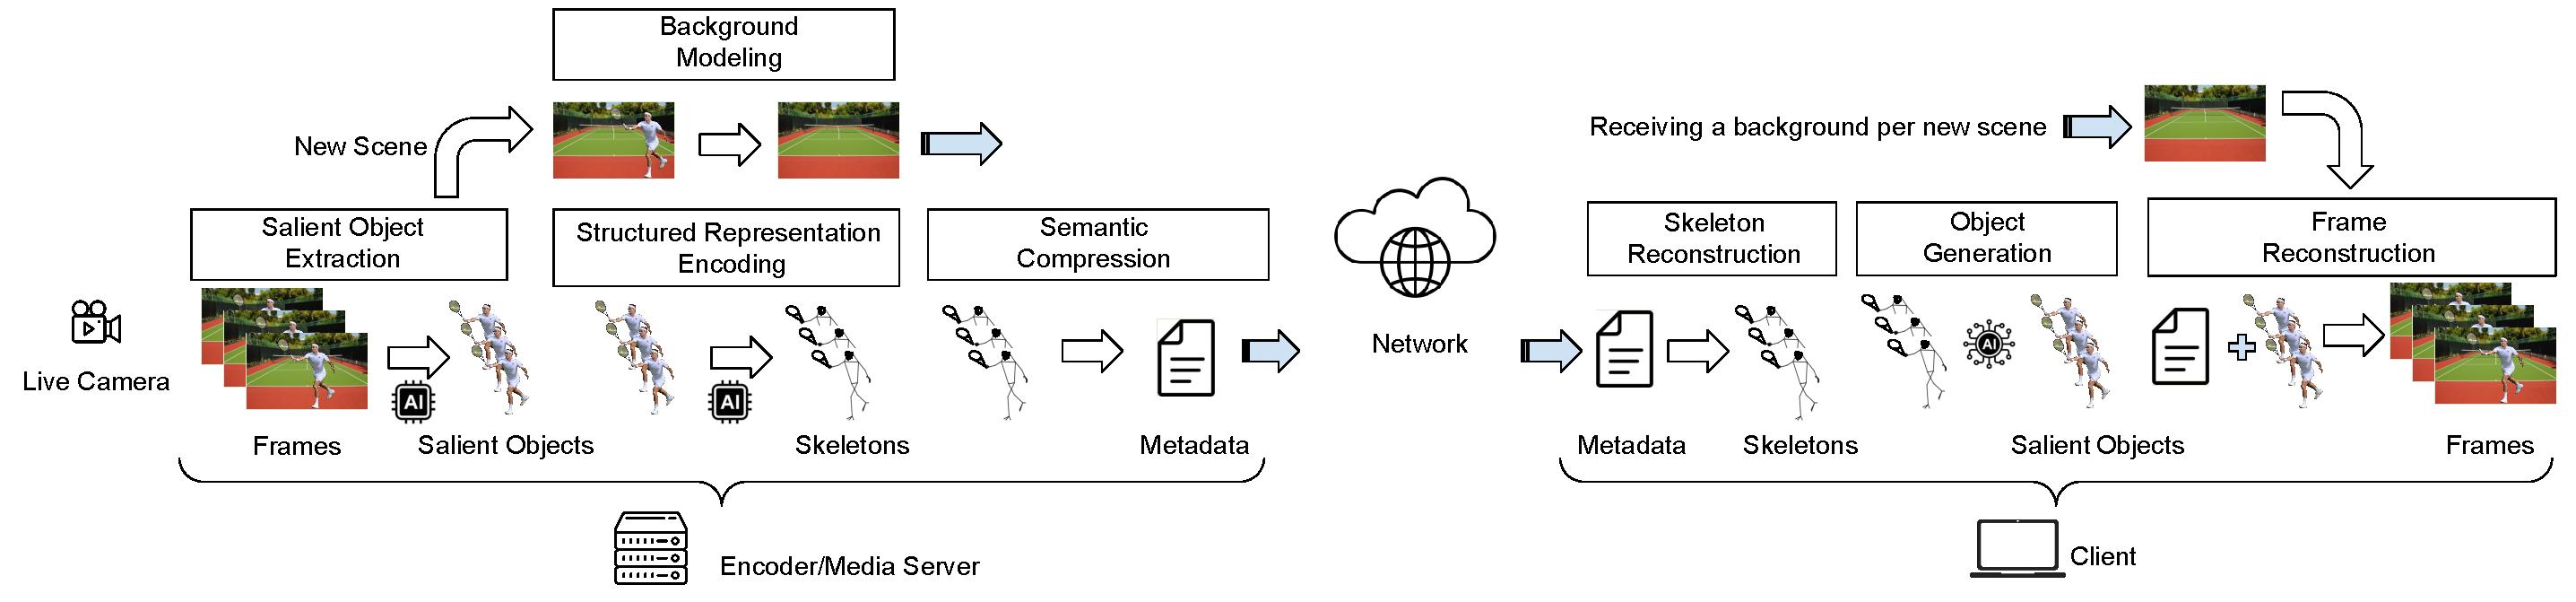
\includegraphics[width=1\linewidth]{figures/PS-overview.pdf}
    \caption{Conceptual overview of PointStream integration into the video streaming pipeline.}
    \label{fig:ps-overview}
\end{figure*}

\subsection{GenAI-based video streaming}
Advances in Generative AI (GenAI) enable impressive progress in image and video synthesis, with models that produce photorealistic scenes and animate static content~\cite{ramesh2021dalle, ho2020ddpm, isola2017pix2pix}. These models learn high-level semantic representations of objects and their motion, which makes them well-suited for applications in video streaming---particularly for reconstructing visual information from compact, abstract encodings. Despite this potential, most generative approaches remain decoupled from real-time streaming pipelines. They typically rely on private datasets and require significant computational resources to train and deploy. As a result, developers mainly use them for offline generation or post-processing, rather than integrating them directly into video compression systems.

Recent attempts explore the possibilities of integrating generative models into video streaming pipelines. For example, ELVIS~\cite{elvis} proposes a client-side inpainting framework that removes low-importance regions from transmitted frames and fills them in using a generative model at the client. This reduces the amount of background elements transmitted over the network. Although innovative, this solution still relies on traditional block-based compression and lacks deeper integration of semantic segmentation and reconstruction. As a result, it does not fully exploit object-level priors or motion-aware representations and treats each block as an isolated unit, rather than as part of a coherent object or action.

While previous work advances compression efficiency, semantic analysis, and generative reconstruction in isolation, these developments largely evolve along parallel tracks. Traditional codecs focus on low-level signal optimization, semantic systems stop at detection without optimized encoding, and generative models remain underutilized within streaming pipelines. The intersection of these trajectories reveals a clear opportunity: a unified framework that combines semantic understanding, compact representation, and generative reconstruction to enable efficient, high-quality video streaming. PointStream emerges in this space, introducing a fully object-based encoding approach that leverages scene semantics to minimize redundancy and uses generative models to reconstruct video content intelligently on the client side.

\section{Problem Description and Motivation}
To evaluate whether our approach brings meaningful improvements, we first establish a baseline by measuring the performance of current state-of-the-art codecs under constrained bandwidth conditions, using a tennis match segment at 4K resolution, a framerate of \SI{50}{\fps}, and \SI{8}{\second} of duration as our test case.
As our reference codec, we select HEVC due to its widespread adoption and high compression efficiency. 
We encode the target video\footnote{\url{https://www.youtube.com/watch?v=7QoKrvOvIGw&t=88s}, last access: 2025-09-18.} at each bitrate among the representations in the Apple HLS bitrate ladder~\cite{AppleHLS}, which results in qualities ranging from \SI{27}{VMAF} at 360p (\vxv{640}{360}) and 145\,Kbps, up to nearly flawless reconstruction at 4K and 11\,Mbps. 

Given the structured nature of many video types, particularly sports, we explore a content-aware alternative that exploits the inherent redundancy in the scene. 
A typical broadcast consists of 
\begin{enumerate*}[label=\textit{(\roman*)}] 
\item a static or predictably moving background (court, audience), and 
\item a few dynamic elements (players, rackets, ball)
\end{enumerate*}.
Instead of encoding all pixels in every frame, we propose a simple yet effective optimization:
\begin{itemize}[topsep=0pt,itemsep=0pt,leftmargin=*]
    \item Extract and store only the moving objects as separate video streams.
    \item Compress and store the background as a single static image.
\end{itemize}
This approach ignores irrelevant motion (\eg minor spectator movements), while significantly reducing bitrate consumption. For our test video, this method reduces the data size by approximately \qty{60}{\percent} compared to the standard 4K HEVC encoding.

Despite these impressive gains, this method still requires encoding full pixel-based representations of moving objects. We observe that players are humans whose motion can be efficiently represented using structured pose information. 
Leveraging this insight, we take an additional step:
\begin{itemize}[topsep=0pt,itemsep=0pt,leftmargin=*]
\item Instead of encoding pixel-level video streams, we extract 2D pose trajectories using a state-of-the-art pose estimator and represent motion as a sequence of keypoints.
\item We employ a lightweight generative model (a cGAN~\cite{isola2017pix2pix}) to reconstruct plausible visual representations of the players conditioned on these pose sequences.
\end{itemize}
This transformation yields another substantial reduction in data size, from the previous \SI{950}{KB} and \SI{1.2}{MB} to \SI{230}{KB} and \SI{294}{MB}, or about \qty{75}{\percent} smaller than the object-video approach, and a total reduction from \SI{4.55}{MB} to \SI{2.92}{MB}, another \qty{36}{\percent} size drop.
% Once more, we forgo to calculate VMAF for these experiments, and instead assume that the client side generative model would be able to replicate players without noticeable artifacts.

We note that these results assume that the perceptual impact of certain approximations is negligible. 
In particular, encoding the background as a static image may reduce objective quality metrics such as VMAF, but we posit that this does not reflect a meaningful drop in perceived quality, given the minimal motion and low saliency of those background elements.
Similarly, in the pose-based reconstruction case, we assume that the generative model produces visually plausible outputs sufficient to maintain perceived fidelity. 
While these assumptions simplify the evaluation, they are reasonable within the controlled scope of this illustrative example.

Although not intended as a rigorous or statistically comprehensive evaluation, this stepwise transformation, from full-frame encoding, to object-background separation, to structured motion-based representation, highlights the potential of a content-aware, human-centric approach. 
These insights directly inform the design of our proposed system, \emph{PointStream}, which generalizes this paradigm into a scalable and modular semantic live streaming pipeline.

%\section{Acknowledgments}
%The financial support of the Austrian Federal Ministry for Digital and Economic Affairs, the National Foundation for Research, Technology and Development, and the Christian Doppler Research Association, is gratefully acknowledged. Christian Doppler Laboratory ATHENA: https://athena.itec.aau.at/

%%
%% The next two lines define the bibliography style to be used, and
%% the bibliography file.
\bibliographystyle{ACM-Reference-Format}
\bibliography{ref}

%%
%% If your work has an appendix, this is the place to put it.
%\appendix

%\section{Section I}

%\subsection{Subsection I}

%Lorem ipsum dolor sit amet, consectetur adipiscing elit.

\end{document}
\endinput
%%
%% End of file `sample-sigconf.tex'.
